% SPDX-License-Identifier: Apache-2.0
%
% What has been built: a few pages on the language, the parts, the core
% and Razboj. Built by //docs:showcase. Every listing is included from
% the tree and the picture is the one Razboj drew.
\documentclass[journal,9pt]{IEEEtran}

\newcommand{\listingsize}{\fontsize{6}{7}\selectfont}
% SPDX-License-Identifier: Apache-2.0
%
% The house preamble, shared by every document in this directory. Loaded
% after \documentclass, before \title. Keeping it in one file is what
% stops two articles drifting apart in font, listing style or figure
% style.
% Computer Modern. IEEEtran selects Times (ptm) by default, so the face has
% to be chosen explicitly.
%
% Latin Modern is the Computer Modern variety used here, and the choice is
% forced rather than aesthetic. Under T1 encoding, plain `cmr` has no Type 1
% outlines unless cm-super is installed, and it is not in the pinned
% distribution, so pdflatex falls back to EC bitmaps and every glyph in the
% PDF becomes a Type 3 font. That was measured: the first build produced a
% document with 10 Type 3 fonts and no Type 1. Latin Modern is Computer
% Modern redrawn with a full T1 repertoire and real .pfb outlines, so the
% same design comes out scalable.
\usepackage[T1]{fontenc}
\usepackage[utf8]{inputenc}
\usepackage{lmodern}
% microtype is not in the pinned TeX distribution. emergencystretch alone
% keeps the two-column measure from producing overfull lines.
\setlength{\emergencystretch}{3em}

\usepackage{amsmath}
\usepackage{amssymb}
\usepackage{amsthm}
\usepackage{booktabs}
\usepackage{array}
% enumitem is not in the pinned TeX distribution; the list spacing below
% does what \setlist would have done.
\usepackage{float}
\usepackage{xcolor}
\usepackage{listings}
\usepackage{tikz}
\usetikzlibrary{arrows.meta,positioning,fit,backgrounds,calc}
\usepackage[hidelinks,bookmarks=true]{hyperref}

% Numbered, definition-style box for a rule the reader is meant to apply.
\theoremstyle{definition}
\newtheorem{rulebox}{Rule}
\newtheorem{example}{Example}

% Unnumbered asides.
\theoremstyle{remark}
\newtheorem*{tip}{Tip}
\newtheorem*{pitfall}{Pitfall}

% Tighter lists, in place of enumitem's \setlist.
\setlength{\topsep}{2pt}
\setlength{\itemsep}{1pt}
\setlength{\parsep}{0pt}

% Code in the running text. The typewriter face under T1 ligates `<<`
% and `>>` into guillemets, so a shift printed as \code{<<} came out as
% a French quotation mark (issue 571). microtype's \DisableLigatures is
% not in the pinned distribution, but the primitive it rests on is
% pdfTeX's own: \pdfnoligatures strips every ligature from the font it
% is given, and the current font inside \texttt is the typewriter face
% at the size in use, so each size is stripped the first time \code
% sets it. Code wants no ligature at all: two quotes are two quotes.
\newcommand{\code}[1]{\texttt{\ifdefined\pdfnoligatures\pdfnoligatures\font\fi #1}}
\newcommand{\term}[1]{\emph{#1}}

% Syntax highlighting. Four roles, distinguishable in colour and still
% distinguishable in greyscale, because an IEEE article gets printed: the
% keyword is the only bold role, the comment is the only italic one, and the
% two remaining roles differ in lightness as well as in hue.
\definecolor{kwblue}{RGB}{20,60,150}
\definecolor{cmtgreen}{RGB}{90,120,90}
\definecolor{strred}{RGB}{150,50,40}
\definecolor{numgray}{gray}{0.45}
\definecolor{framegray}{gray}{0.70}
\definecolor{bgshade}{gray}{0.97}
% A darker fill for figure cells. The listing background has to stay very
% light to keep code readable; a figure cell has to be clearly shaded or the
% distinction it draws is invisible in print.
\definecolor{cellshade}{gray}{0.90}

% The listing size is the document's choice, because it depends on the
% column: a two-column article sets `\listingsize` to 6pt and keeps its
% listings within 70 columns, or to 5.6pt when it includes source that
% rustfmt sets at 80, which is what fits a column's frame (issue 1061);
% a one-column document keeps the body size and includes source files
% at 80. `//docs:frame_test` checks every listing line against its frame. Lines are never broken; a line that does not fit
% overflows the frame, which is visible, rather than wrapping, which is
% not.
\providecommand{\listingsize}{\scriptsize}

% `'` is deliberately not a string delimiter: the language uses it for loop
% labels, as Rust does, so treating it as a quote would swallow the rest of
% the line.
\lstdefinestyle{txhdl}{
  basicstyle=\ttfamily\listingsize,
  keywordstyle=\bfseries\color{kwblue},
  commentstyle=\itshape\color{cmtgreen},
  stringstyle=\color{strred},
  numberstyle=\tiny\color{numgray},
  morekeywords={mod,use,pub,const,type,struct,enum,trait,impl,fn,async,let,mut,
    match,if,else,loop,while,for,in,break,continue,return,as,await,
    module,bus,channel,transaction,protocol,pipeline,flow,seq,config,
    port,stage,pipe,instance,connect,bind,tag,domain,blackbox,foreign,
    property,role,signal,handler,true,false,
    sequence,interface,modport,implements,package,import,var,wire,func,proc,
    case,default,next,fork,branch,join,state,fsm},
  morecomment=[l]{//},
  morestring=[b]",
  showstringspaces=false,
  columns=fullflexible,
  keepspaces=true,
  breaklines=false,
  % Framed, so a listing is bounded rather than floating in the column.
  frame=single,
  rulecolor=\color{framegray},
  framesep=3pt,
  backgroundcolor=\color{bgshade},
  xleftmargin=3pt,
  xrightmargin=3pt,
  aboveskip=6pt,
  belowskip=6pt,
  % Every listing is numbered and captioned, so it can be referred to by
  % number. `caption` without `float` numbers the listing and leaves it
  % where it was written, which is what a listing in running prose needs.
  captionpos=b,
  abovecaptionskip=2pt,
  belowcaptionskip=6pt,
}

% Figures drawn as text. Framed the same way, and with the highlighting
% switched off, because a box-and-arrow diagram is not code and half its
% words turning blue reads as an accident. Setting a style adds keys rather
% than clearing the ones already set, so the three roles are neutralised by
% hand rather than by leaving them out. Program output is printed in this
% style too, and a netlist's assignment can run past the frame, so a line
% that does not fit is broken and the rest indented; source never is.
\lstdefinestyle{ascii}{
  basicstyle=\ttfamily\listingsize,
  keywordstyle=\ttfamily,
  commentstyle=\ttfamily,
  stringstyle=\ttfamily,
  columns=fullflexible,
  keepspaces=true,
  breaklines=true,
  breakindent=2em,
  frame=single,
  rulecolor=\color{framegray},
  framesep=3pt,
  backgroundcolor=\color{bgshade},
  xleftmargin=3pt,
  xrightmargin=3pt,
  aboveskip=6pt,
  belowskip=6pt,
}
\lstset{style=txhdl}

% House TikZ styles. `shorten` lives on the arrow styles rather than on each
% arrow, so every arrow in the document gets the gap, including ones added
% later. TikZ clips a path at a node's border, so without it an arrowhead
% butts against the box with no gap at all. Keep `node distance` well above
% twice the shorten, or the arrow shrinks to nothing.
\tikzset{
  box/.style={draw,rounded corners=2pt,align=center,inner sep=4pt,
              font=\footnotesize},
  boxf/.style={box,fill=bgshade},
  lbl/.style={font=\scriptsize\itshape,align=center},
  fl/.style={-{Stealth[length=4pt]},shorten >=2.5pt,shorten <=2.5pt},
  fld/.style={fl,dashed},
}


% The contents list: the class gives a section's number 2.75em, which
% a Roman numeral past thirty overruns onto the title, so the box is
% wider here, and a subsection's entry starts where a title does.
\makeatletter
\def\l@section#1#2{\addpenalty{\@secpenalty}\addvspace{1.0em plus 1pt}%
    \@tempdima 5.75em \begingroup \parindent \z@ \rightskip \@pnumwidth%
    \parfillskip-\@pnumwidth {\bfseries\leavevmode #1}\hfil\hbox to\@pnumwidth{\hss #2}\par%
    \endgroup}
\def\l@subsection{\@dottedtocline{2}{5.75em}{5em}}
\def\l@subsubsection{\@dottedtocline{3}{10.75em}{5.5em}}
\makeatother

\usepackage{graphicx}

\InputIfFileExists{buildstamp.tex}{}{}
% The numbers the ASIC run produced, written by the run itself.
\input{asic_counts.tex}
\providecommand{\buildstamp}{Draft build (outside the Bazel flow).}

\title{TxHDL: What Has Been Built}

\author{Filip Filmar and Dragiša Janković%
\thanks{Both authors are independent. Filip Filmar is the
corresponding author, at f@hdlfactory.com; Dragiša Janković is
reached at linkedin.com/in/dragisa-jankovic.}%
\thanks{A summary of the complete implementation for readers seeking an
architectural overview before consulting the detailed monograph. Every
technical claim maps directly to an automated target in the project
repository \code{HDL/txhdl}; the cover document, \code{//docs:cover},
catalogues the twenty-three companion reports.}%
\thanks{The authors used a large language model, Claude, as an
assistant in exploring concepts and in drafting and constructing
the documents and implementations; every repository commit documents
this collaboration and includes the prompt sequence verbatim.}%
\thanks{\buildstamp}}

\markboth{TxHDL: What Has Been Built}{Filmar and Janković: TxHDL: What Has Been Built}

\begin{document}
\maketitle

\section{The Rule}

TxHDL is a hardware description language implemented purely as a Rust
library. Its architecture emerged by systematically stripping away every
redundant construct that the host language already provides. A transaction is a
native \code{struct}; a hardware module is a \code{struct} implementing the
\code{Unit} trait; a synchronous pipeline is an \code{async fn}; a parameter
configuration is a trait constraint. A clock is an affine type, paired
implicitly with its synchronous reset: every emitted netlist binds one, every
lowered sub-unit joins its parent domain, and no unit pollutes its interface
with explicit reset wiring---sparing approximately 127 individual \code{.run}
invocation sites. Under reset assertion, every register restores its initial
state and every communication channel empties. The host compiler, \code{rustc},
serves as front-end parser and design-rule checker: driving a wire from
multiple sources violates affine move semantics, crossing clock domains outside
an explicit \code{ChanCdc} primitive triggers a static type mismatch, and
registering a cycle in purely combinational logic is syntactically prohibited
because a synchronous \code{fn} admits no \code{.await} expression.

What remains is a unit, and every unit is a synthesizable netlist.
Listing~\ref{lst:w-unit} shows a complete example: a three-bit counter that
pulses once every eight cycles while asserted. The \code{\#[lower]} procedural
attribute derives cycle-equivalent Verilog and VHDL definitions alongside the
Rust implementation, and hermetic build actions co-simulate both HDL netlists
against the Rust execution trace on every run.

\lstinputlisting[rangebeginprefix=//\ begin\{,rangebeginsuffix=\},%
rangeendprefix=//\ end\{,rangeendsuffix=\},includerangemarker=false,%
linerange=unit-unit,caption={A unit, whole. Its netlist and its
waveform are on the cheat sheet, \code{//docs:cheatsheet}.},%
label={lst:w-unit}]{lib/examples/ex_cheat.rs}

\section{What Is In It}

Table~\ref{tab:w-units} details the hardware units lowered to Verilog and VHDL,
while Table~\ref{tab:w-systems} catalogues the integrated systems composed from
them. These tables reflect the documented corpus baseline; ongoing peripheral
development is tracked via active repository issues. In aggregate, the
implementation spans 94\,581 physical lines of Rust: 18\,484 across runtime
abstractions and procedural macros, 26\,512 in reusable subsystem parts,
18\,113 distributed across 121 compiled examples, 25\,927 comprising the
Vreteno processor and its FPGA board envelope, and 5\,545 spanning the Razboj
GPU, DDR3 controller, Ethernet MAC, HDMI rasterizer, PCIe bridge, and unified
SoC.

\begin{table}[htbp]
\caption{The lowered units, and which netlists are simulated.}
\label{tab:w-units}
\centering\footnotesize
\begin{tabular}{@{}p{0.50\columnwidth}lp{0.22\columnwidth}@{}}
\toprule
Unit & Where & Simulated \\
\midrule
The channel, a buffer of two & runtime & inside a parent \\
Buffer; FIFO & parts & both \\
A channel across two clocks & parts & yes \\
Memory engines, 3; tie-offs, 2 & parts & the engines \\
A scanout from memory: two lines a line ahead, their fetch, and the video peripheral it joins & parts & all three \\
Stations of 2 to 10 inputs & parts & 2 and 3 \\
An AXI router, one unit for N peripherals & parts & 3 \\
An AXI arbiter, one unit for 2 to 8 hosts & parts & 2 \\
AXI host and peripheral trackers & parts & both \\
An AXI-Lite bridge, one unit for N peripherals; a slot split in two & parts & 1 and 2; the split in a parent \\
AXI to Wishbone bridge & parts & yes \\
AXI host pins to the link's channels & parts & yes \\
The link's channels to a peripheral's AXI pins & parts & yes \\
An interrupt controller, one unit for 1 to 31 sources & parts & 3 \\
Sv32 translation: fetch and data TLBs, a walker that never writes & parts & yes \\
Network node, switch, 2 bridges; a mesh of nodes & parts & the mesh \\
Pins; SPI; I2C; MDIO; SD; Ethernet's five; HDMI's two & parts & all twelve \\
The RISC-V debug transport, behind \code{BSCANE2}, and its bridge & parts & the transport \\
Words to frames and back; a frame's length & parts & all three \\
System control: identity, cause, reset & parts & yes \\
Watchdog: a countdown, a key, a window & parts & yes \\
Four modulated outputs, shadowed duties & parts & yes \\
A trace buffer, the last N entries & parts & yes \\
An entropy source: eight rings, two health tests, debiased, captured & parts & yes \\
A tee and a check, for running one thing twice & parts & both \\
A flash read as memory, mode 0 only & parts & both \\
The configuration flash through \code{STARTUPE2}, write enable refused & parts & yes \\
A peripheral written as software, behind a channel & parts & both \\
Its wire: each transaction one Ethernet frame & parts & both \\
Vreteno, a hart with its Sv32 unit; boot and data memory, timer, serial port & \code{cpu} & four of five \\
The board, one unit of units, with DDR3 & \code{cpu} & under Vivado \\
Rasteriser; framebuffer & \code{gpu} & both \\
PCIe BAR registers; the BAR as one unit & \code{pcie} & not yet \\
The examples' own units & examples & 79, in 62 files, all 62 \\
\bottomrule
\end{tabular}
\end{table}

\begin{table}[htbp]
\caption{The systems the build assembles, and what checks each.}
\label{tab:w-systems}
\centering\footnotesize
\begin{tabular}{@{}p{0.22\columnwidth}p{0.36\columnwidth}p{0.29\columnwidth}@{}}
\toprule
System & Made of & Checked by \\
\midrule
Vreteno & core, router, 4 devices & model, 6 netlists \\
A lockstep pair & 2 cores, 3 tees, 3 checks & 8 programs, a fault \\
Razboj, a GPU & rasteriser, link, memory & model, 2 netlists \\
The AXI link & host and peripheral & 2 netlists \\
The AXI router & 1 host, 3 peripherals & its netlist \\
The AXI-Lite bridge & 1 host, 2 banks & 3 netlists \\
A lattice & 4 nodes, both bridges, RAM & 8 tests \\
A mesh & 6 nodes in one unit & its netlist \\
The SoC & core, GPU, RAM, serial & its run \\
Composition & station, stream ALU & its netlist \\
The board & core, 8 devices, DDR3, a JTAG host, the debug transport & 3 runs, OpenOCD and gdb, Vivado, the cable \\
Ethernet & the MAC, the board's PHY & on the board \\
Video & HDMI, its I2C, the board & on the board \\
PCIe & XDMA endpoint, pins, registers & a run, Vivado \\
The flagship & board, Ethernet, video, Razboj, in one part & the board, routed \\
On silicon & Vreteno, Yosys, OpenROAD & routed, no DRC \\
\bottomrule
\end{tabular}
\end{table}

\section{Vreteno, a Core}

Vreteno is an RV32IMAC processor core implementing an in-order fetch, execute,
and writeback pipeline, with sequential multi-cycle integer multiplication and
division, privileged machine control registers, an architectural timer, and
vectored external interrupts. The microarchitecture is validated in lockstep
against an authoritative software ISA reference model on every cycle: program
counter progression, all 31 general-purpose registers, and privileged CSR
state must match identically across every instruction retirement, verified
across deterministic benchmark binaries and 64 randomised instruction
sequences. Outside local boot memory, instruction fetch traverses a 16\,KB
direct-mapped cache, sustaining 3.3 cycles per instruction on loop execution
from system memory, compared to 14.7 cycles per instruction when fetching
unbuffered across the system bus. The core integrates supervisor and user
privilege modes alongside an Sv32 memory management unit featuring dual 8-entry
instruction and data TLBs; targeting the physical development board, it boots a
full Linux distribution to an interactive shell within thirty seconds of image
receipt.

The design operates seamlessly on silicon targets. Lowered RTL netlists are
synthesized hermetically through Vivado targeting an Alinx AX7A200B FPGA; upon
boot, the hardware UART emits the expected simulation string---\code{OK}---and
faithfully echoes interactive character input. The identical netlist is
lowered to an open 45\,nm standard-cell library using pinned releases of Yosys
and OpenROAD, yielding a square die of \asicdie\,$\mu$m per side meeting a
closed clock frequency of \asicfreq\,MHz with \asicdrc{} design-rule
violations. This physical layout represents an automated demonstration; the
remaining steps required for foundry tapeout are catalogued in
\code{//docs:tapeout}.

System interconnection is built upon AXI4. Every subordinate device behaves as
an AXI peripheral, mapped by an address-decoding router. On the evaluation
board, this fabric addresses 1\,GB of DDR3 SDRAM via a vendor memory-interface
controller integrated as a foreign module: the sole external component wired
rather than directly authored in TxHDL. Figure~\ref{fig:s-board} illustrates
the complete board topology.

\begin{figure}[htbp]
\centering
\resizebox{\columnwidth}{!}{%
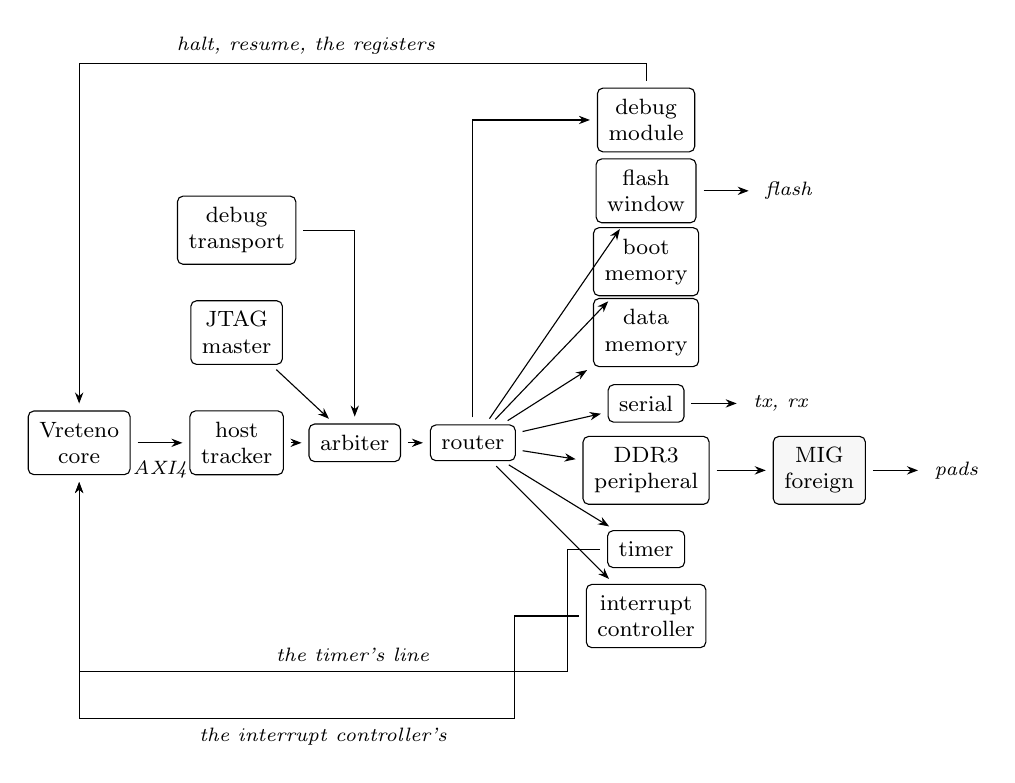
\begin{tikzpicture}[x=1cm, y=1cm, every node/.style={font=\scriptsize}]
  \node[box] (cpu) at (0,0) {Vreteno\\core};
  \node[box] (host) at (2.0,0) {host\\tracker};
  \node[box] (arb) at (3.5,0) {arbiter};
  \node[box] (jtag) at (2.0,1.4) {JTAG\\master};
  \node[box] (dtm) at (2.0,2.7) {debug\\transport};
  \node[box] (rt) at (5.0,0) {router};
  \node[box] (rom) at (7.2,2.3) {boot\\memory};
  \node[box] (dmem) at (7.2,1.4) {data\\memory};
  \node[box] (uart) at (7.2,0.5) {serial};
  \node[box] (ddr) at (7.2,-0.35) {DDR3\\peripheral};
  \node[boxf] (mig) at (9.4,-0.35) {MIG\\foreign};
  \node[box] (tim) at (7.2,-1.35) {timer};
  \node[box] (plic) at (7.2,-2.2) {interrupt\\controller};
  \node[box] (dm) at (7.2,4.1) {debug\\module};
  \node[box] (fw) at (7.2,3.2) {flash\\window};
  \draw[fl] (cpu) -- node[lbl, below=3pt] {AXI4} (host);
  \draw[fl] (host) -- (arb);
  \draw[fl] (jtag) -- (arb);
  \draw[fl] (dtm.east) -| (arb.north);
  \draw[fl] (arb) -- (rt);
  \draw[fl] (rt) -- (rom);
  \draw[fl] (rt) -- (dmem);
  \draw[fl] (rt) -- (uart);
  \draw[fl] (rt) -- (ddr);
  \draw[fl] (rt) -- (tim);
  \draw[fl] (rt) -- (plic);
  \draw[fl] (rt.north) |- (dm.west);
  \draw[fl] (rt) -- (fw);
  \draw[fl] (dm.north) -- ++(0,0.3) -| (cpu.north)
    node[lbl, above, pos=0.3] {halt, resume, the registers};
  \draw[fl] (ddr) -- (mig);
  \draw[fl] (mig.east) -- ++(0.75,0) node[lbl, right] {pads};
  \draw[fl] (uart.east) -- ++(0.75,0) node[lbl, right] {tx, rx};
  \draw[fl] (fw.east) -- ++(0.75,0) node[lbl, right] {flash};
  % The two lines the core waits on run in lanes of their own, below
  % every box, so neither crosses one.
  \draw[fl] (tim.west) -- ++(-0.5,0) |- (0,-2.9)
    node[lbl, above, pos=0.72] {the timer's line} -| (cpu.south);
  \draw[fl] (plic.west) -- ++(-0.9,0) |- (0,-3.5)
    node[lbl, below, pos=0.72] {the interrupt controller's} -| (cpu.south);
\end{tikzpicture}}
\caption{The board: the core, its tracker, the JTAG master and the
debug transport, which share the bus with it through the arbiter, the router that decides by
address, and the eight peripherals behind it. The DDR3 controller is a
foreign module, wired rather than written; the serial port reaches two
pins, the flash window reaches the configuration flash, the interrupt
controller and the timer reach the core's two lines, and the debug
module reaches its halt, resume and registers.}
\label{fig:s-board}
\end{figure}

\section{The AXI Link}

A native channel transports a single transaction. The AXI4 protocol
coordinates five independent channels that maintain semantic validity only in
concert. The TxHDL library therefore abstracts the interconnect as a cohesive
link: invoking \code{axi()} instantiates all five constituent channels
atomically, returning paired host and peripheral endpoints analogously to
\code{chan()} yielding connected sender and receiver handles.

A host client initiates a burst request and awaits its corresponding response
out of order. A peripheral client receives complete transactional descriptors
and commits responses asynchronously from whichever process finishes the
underlying work. Client implementations never manipulate raw channel handshake
signals, track burst beat counters, or manage transaction ID tags directly.
Autonomous protocol trackers situated at each link boundary enforce protocol
invariants, permitting intermediate routers to steer traffic without altering
client code.

\section{A Network}

While an AXI router aggregates multiple peripherals beneath a single host,
multi-host, multi-peripheral fabrics require a packet-routed topology. TxHDL
implements a scalable 2D torus/mesh network-on-chip: each routing node couples
bidirectional links to its cardinal neighbours with a fifth injection/ejection
port attached to an AXI protocol bridge. Every physical link multiplexes two
virtual channels---one dedicated to requests and one to responses---precluding
request buffers from saturating the fabric and stalling the response packets
required to drain them. Dimension-order routing guarantees structural freedom
from routing deadlocks without virtual-channel reassignment.

Endpoint modules remain completely oblivious to the packetised fabric. Hosts
issue standard AXI bursts and await responses; peripherals consume transactions
and commit replies transparently. The network bridge manages transaction ID
namespace remapping: because transaction IDs are local to the originating host,
peripheral bridges translate request IDs dynamically, caching the source
coordinates and original transaction tag to route replies back to their origin.

In demonstration, Vreteno, the Razboj GPU, shared SRAM, and a UART peripheral
occupy the four nodes of a $2\times 2$ mesh (Figure~\ref{fig:s-noc}). Working
concurrently, the CPU computes vertex coordinates for a rotating icosahedron
and writes the resulting display list into shared memory over the network. The
Razboj rasteriser detects the list, traverses the geometry, and renders pixels
into the frame buffer. Traversal of the packet mesh imposes an approximately
two-fold latency penalty over a direct point-to-point link, representing the
routing overhead of a single-flit-per-cycle distributed fabric.

\begin{figure}[htbp]
\centering
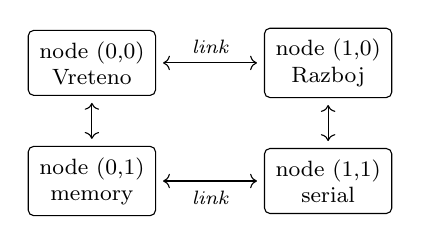
\begin{tikzpicture}[x=1cm, y=1cm, every node/.style={font=\scriptsize}]
  \node[box] (n00) at (0,1.5) {node (0,0)\\Vreteno};
  \node[box] (n10) at (3.0,1.5) {node (1,0)\\Razboj};
  \node[box] (n01) at (0,0) {node (0,1)\\memory};
  \node[box] (n11) at (3.0,0) {node (1,1)\\serial};
  \draw[fl, <->] (n00) -- node[lbl, above] {link} (n10);
  \draw[fl, <->] (n01) -- node[lbl, below] {link} (n11);
  \draw[fl, <->] (n00) -- (n01);
  \draw[fl, <->] (n10) -- (n11);
\end{tikzpicture}
\caption{The system on a two by two lattice: the core, the rasteriser,
the memory they share and the serial port, one to a node. Every link
is two virtual channels, one for requests and one for responses, and
each node's fifth port is the bridge that puts AXI on the network.}
\label{fig:s-noc}
\end{figure}

\section{Razboj, a GPU}

\begin{figure}[htbp]
\centering
\includegraphics[width=0.36\columnwidth]{scene.png}
\caption{Eight display list entries, drawn by the rasteriser, written
into memory over AXI, read back and written out as this file.}
\label{fig:w-scene}
\end{figure}

Figure~\ref{fig:w-scene} was rendered directly by synthesised hardware logic.
The Razboj rasteriser traverses the axis-aligned bounding box defined by each
display-list primitive at one pixel per clock cycle, evaluating three edge
functions incrementally. Pixel spans along each scanline are committed to
memory through AXI burst writes of up to 16 beats, masking write strobes for
sample points falling outside triangle boundaries. The receiving framebuffer
operates as a memory controller across the bus link. Both modules are fully
lowerable units, and regression suites co-simulate their gate netlists against
the software model that produced the reference render. Within the flagship SoC,
the rasteriser operates as a second bus-mastering host: software populates a
display list in DDR3 memory, asserts a doorbell register on the control page,
and Razboj autonomously paints the frame buffer scanned out to the physical
display.

\section{Parts}

In TxHDL, a reusable part is standard hardware implemented strictly within the
synthesizable language subset. Modules are subjected to the same lowering and
verification rules as custom designs; the standard library incorporates no
magic compiler primitives hidden from the user. Out-of-order execution
primitives include parameterised reservation stations that aggregate operands
arriving asynchronously across disparate channels, firing execution upon
complete dependency resolution.

The component library radiates outward from the central bus: a full-duplex
Ethernet MAC; an HDMI video timing generator paired with a dedicated I2C
transmitter for encoder initialization; a general-purpose I2C master; GPIO
pads; an SPI master; a system controller reporting active design identity and
reset provenance; a windowed watchdog timer that forces a reset when software
heartbeats lapse; and an AXI-to-Wishbone bridge enabling seamless integration of
legacy IP cores.

The bus ecosystem accommodates bidirectional complexity. Address routers steer
requests from a single host across multiple subordinate endpoints; arbiters
multiplex multiple competing hosts onto a single peripheral channel using fair
round-robin scheduling, prepending host tags so responses return
deterministically to their initiator. The introduction of this bus arbiter
unlocked multi-master concurrency, allowing Razboj, DMA controllers, and
secondary processors to coexist alongside the primary core.

\begin{figure}[htbp]
\centering
\input{paper_cheat_timing.tex}
\caption{The unit of Listing~\ref{lst:w-unit}, running. The build drew
this from the trace that same run wrote, and generated a testbench
from it that replays the netlist.}
\label{fig:w-wave}
\end{figure}

\begin{figure}[htbp]
\centering
\resizebox{\columnwidth}{!}{%
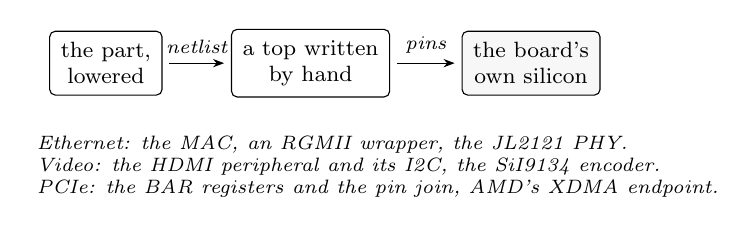
\begin{tikzpicture}[x=1cm, y=1cm, every node/.style={font=\scriptsize}]
  \node[box] (part) at (0,0) {the part,\\lowered};
  \node[box] (top) at (2.6,0) {a top written\\by hand};
  \node[boxf] (out) at (5.4,0) {the board's\\own silicon};
  \draw[fl] (part) -- node[lbl, above] {netlist} (top);
  \draw[fl] (top) -- node[lbl, above] {pins} (out);
  \node[lbl, align=left, anchor=north west] at (-1.0,-0.8)
    {Ethernet: the MAC, an RGMII wrapper, the JL2121 PHY.\\
     Video: the HDMI peripheral and its I2C, the SiI9134 encoder.\\
     PCIe: the BAR registers and the pin join, AMD's XDMA endpoint.};
\end{tikzpicture}}
\caption{The three designs that reach the board's own silicon have one
shape: a lowered part, a top written by hand for the clocking and the
pins, and a chip on the far side of them. Each goes through Vivado to
a bitstream; what has run on the board is in Table~II.}
\label{fig:s-boards}
\end{figure}

\section{From an Empty Directory}

A developer equipped only with Bazelisk and Git can draft five concise
configuration files to build, simulate, and lower an LED blinky design to
synthesizable Verilog. The project is consumed via standard external repository
rules pinned to an immutable git commit. Continuous integration builds this
standalone tutorial design against the active working tree to ensure external
examples never suffer bitrot. Every toolchain in Table~\ref{tab:w-tools} is
fetched and verified hermetically by Bazel---either via cryptographic checksum
or compiled directly from source---with the sole exception of AMD Vivado, which
requires authenticated vendor licensing. No supplementary toolchains are
installed manually on local workstations or CI runners.

\begin{table}[htbp]
\caption{The toolchains the build fetches.}
\label{tab:w-tools}
\centering\footnotesize
\begin{tabular}{@{}ll@{}}
\toprule
Toolchain, and what the build uses it for & Version \\
\midrule
Rust, for the host and for the core & 1.90.0, nightly \\
GNU C and C++, for the core & 14.2.0 \\
LLVM C and C++, for the host & 20.1.8 \\
\code{nvc}, to simulate VHDL & from source \\
Verilator, to simulate Verilog & 5.046, prebuilt \\
Vivado, Artix-7, to synthesise & 2025.2 \\
Yosys and OpenROAD, to lay out & pinned packages \\
SymbiYosys and z3, to prove & 0.52; 4.13.3 \\
TinyTeX, for the documents & pinned \\
Go, for the serial watcher & 1.25.1 \\
OpenOCD, to debug over JTAG & 0.12.0 \\
gdb, to load a program and break in it & 16.3 \\
Two waveform converters, for figures & pinned \\
\end{tabular}
\end{table}

\section{How It Is Checked}

No behavior is validated by casual inspection. Every example is a standalone
executable program compiled and executed by Bazel; its console output and signal
dumps are embedded directly into documentation from build artifacts, preventing
divergence between text and reality. Each lowered module in
Table~\ref{tab:w-units} is verified twice in parallel: as VHDL under \code{nvc}
and as Verilog under Verilator, with port transitions asserted against the
golden trace captured during native Rust simulation. Running \code{bazel test
//...} invokes 462 automated targets, including 246 co-simulated netlists, the
golden ISA CPU model, bare-metal software test programs, in-circuit debug
sessions linking OpenOCD and GDB over the JTAG transport, Razboj graphics
regressions, peripheral unit tests, full SoC integration runs, ten formal
property proofs, automated diagram boundary checks, and compiler toolchains.
Fifteen long-running targets are reserved for manual or nightly qualification:
optimized board simulations, DDR3 memory controller verification under the
Vivado simulator, standalone and root-port PCIe endpoint regressions, randomized
AXI link fuzzing, datasheet completeness audits, bitstream flash preservation
checks, and four end-to-end Linux boots verifying networking and interactive
shell responsiveness.

Simulation tests validate targeted input stimuli; formal verification proves
invariant properties across all reachable states. Hardware modules declare
safety invariants via \code{check!}, environment constraints via
\code{assume!}, and reachability targets via \code{cover!}. The
\code{formal\_test} rule extracts netlist assertions into SymbiYosys running
against pinned Yosys: Property Directed Reachability (\code{abc pdr}) proves
unbounded safety invariants for all valid input combinations, intentional bug
injections verify that faulty logic triggers counterexamples, Z3 isolates
failing execution cycles, and cover runs generate witness traces demonstrating
target reachability. Every reset-conditioned unit is formally proved to suppress
checks during reset assertion. These ten formal suites complete within seconds,
as documented in \code{//docs:prove}.

Similarly, every factual claim regarding host language type semantics is backed
by standalone compiler probes preserved in the tree, retaining negative
outcomes alongside positive validations to document compiler diagnostics.

\section{What Is Not Done}

A lowered netlist wire may be assigned a canonical name distinct from its
lexical Rust binding, recorded as an explicit rename comment within the
generated Verilog and VHDL. Every valid Rust \code{let} statement is now
accepted without restriction. The Vreteno core executes arbitrary unbuilt code
fetched from system memory beyond its internal boot ROM, and that boot ROM
resides on the AXI bus as read-only memory; however, off-chip instruction cache
misses stall the execution pipeline until the read completes. The
network-on-chip fabric refuses wrapping AXI burst transfers, decomposing
incrementing bursts into single-beat transactions across the mesh. In graphics,
the Razboj rasteriser lacks depth buffering, barycentric perspective
interpolation, and texture filtering. Each of these architectural boundaries is
tracked as an active issue in the repository rather than deferred in prose.

\end{document}
